%%%%%%%%%%%%%%%%%%%%%%%%%%%%%%%%%%%%%%%%%%%%%%%%%%%%%%%%%%%%%%%%%%%%%%%%%%%%%
%% Descr:       Vorlage für Berichte der DHBW-Karlsruhe, Ein Kapitel
%% Author:      Prof. Dr. Jürgen Vollmer, vollmer@dhbw-karlsruhe.de
%% $Id: kapitel2.tex,v 1.5 2017/10/06 14:02:51 vollmer Exp $
%%  -*- coding: utf-8 -*-
%%%%%%%%%%%%%%%%%%%%%%%%%%%%%%%%%%%%%%%%%%%%%%%%%%%%%%%%%%%%%%%%%%%%%%%%%%%%%%%

\chapter{Konzeption}
\label{chap:Konzeption}
In diesem Kapitel wird das erarbeitete Konzept dieser Ausarbeitung dargelegt. Unter dessen die Überlegungen zu einzelnen 
Arbeitsschritten und dem grundsätzlich angedachten Aufbau des Projekts, sowie Entscheidungs- und Beweggründe wieso bestimmte 
Technologien gewählt wurden. Zu Beginn wird auf die Einsatzmöglichkeiten (\ref{chap:Arbeitsumgebung}), in der die Applikation Anwendung 
finden könnte, eingegangen. Anschließend werden die Grundgedanken zu den einzelnen Phasen, Scan-Phase (\ref{chap:Scan-Phase}) und 
Visualisierungs-Phase (\ref{chap:Visualisierungs-Phase}) des Systems erläutert, was sie beinhalten und wie sie funktionstechnisch 
angedacht sind. Mit den zugrundeliegenden Informationen wird auf das Architekturkonzept (\ref{chap:Architekturkonzept}), sowie auf das 
Softwarekonzept (\ref{chap:Architekturkonzept}) eingegangen. Des Weiteren werden die Hintergründe der Wahl des AR-Frameworks 
(\ref{chap:Auswahl des AR Frameworks}) aufgezeigt und abschließend wird noch das konzipierte und prototypische Datenmodell 
(\ref{chap:Datenmodell}) dargelegt.

\section{Anwendungsumfeld}
\label{chap:Arbeitsumgebung}
Bei der Konzeption wird darauf Rücksicht genommen, die Anwendung möglichst so zu planen, dass der Einsatzort zu Anfang nicht zwingend 
maßgeblich ist. Dies bedeutet, dass je nach Anwendungsfall die Applikation angepasst werden kann. Allerdings sind für das 
Unterstützungssystem ausschließlich Produktionshallen, eventuell auch Logistik- oder Lagerhallen, vorgesehen. Durch die individuelle 
Möglichkeit des Umgebungsscans ist die Applikation anfangs nicht an festgelegte Orte gebunden. Damit wird zum Ausdruck gebracht, dass der 
Umgebungsscan flexibel durchgeführt werden kann, da keine Anforderungen an die Umgebung gestellt sind. Die darauf aufbauende 
Visualisierungs-Phase ist demnach abhängig von dem Ort, indem der Scan durchgeführt wurde und kann nicht anderweitig, in anderen Hallen, 
eingesetzt werden. 
\\ 
\linebreak
Ein mögliches Anwendungsumfeld dieser Applikation wären die Räumlichkeiten der nahe bei cjt Systemsoftware AG angesiedelten Siemens AG. Neben 
der Vielzahl an gemeinsamen Projekten, wäre dies eine weitere Kooperation mit der Siemens AG und würde eine unterstützende Maßnahme einleiten. 
\pagebreak
\section{Scan-Phase}
%Objekterkennung /
\label{chap:Scan-Phase} %der Aufgabe
Die Definition der Scan-Phase ist entscheidend für die Konzeption und Umsetzung der Architektur- und Softwarekonzeption. 
Anhand der dabei entstehenden Anforderungen und Zielsetzungen kann die Konzeption ausgelegt und erarbeitet werden. Dieser Abschnitt widmet 
sich der expliziten theoretischen Erläuterung dieser Phase und somit auch einer der beiden Kernfunktionen dieses Softwaresystems.
\\ 
\linebreak
Der Nutzer hält ein Smartphone oder Tablet in der Hand und steht am Eingang der Räumlichkeit. An diesem Punkt wird der Scan-Vorgang gestartet. 
Mittels Smartphone-Kamera hat der Nutzer die Möglichkeit, das Umfeld zu scannen. Dabei wird am Anfang der Startpunkt als Nullpunkt, bzw. 
als Ursprungskoordinaten des erstellten Koordinatensystems der Umgebung, festgelegt. Der Nutzer kann sich frei im Raum bewegen und ist lediglich 
durch das Halten des Smartphones eingeschränkt. Während der Aufnahme wird anhand der im Smartphone integrierten Kamera und 
Sensoren unter Verwendung der Sensordaten ein Modell erstellt, welches die Umgebung virtuell repräsentiert. Dabei wird das Modell auf 
einem dreidimensionalen Koordinatensystem widergespiegelt, um Position, Blickrichtung und Höhe des zu erstellenden Objektes festzuhalten. 
So kommt das \acl{SLAM} Verfahren (siehe Abschnitt \ref{chap:SLAM}) zum Einsatz, das das Smartphone genauestens räumlich lokalisiert und 
gleichzeitig mapped. Dies bedeutet, dass anhand der generierten Sensordaten eine Analyse der Informationen stattfindet und daraus eine 
virtuelle Karte des Raums erstellt wird. Dadurch kann das Gerät die Realität wiedergeben. Anhand der Informationen, die durch
Gegenstände, Wände und dem Boden grundlegend gegeben sind, resultieren die Anhaltspunkte der virtuellen Umgebung. 
\\ 
Dem Nutzer soll die Möglichkeit geboten sein, Objekte an denen vom Anwender vorgesehenen Positionen platzieren zu können. Die Objekte werden 
dann, anhand der durch das \acs{SLAM}-Verfahren zugrundeliegenden Informationen, an der virtuellen Position erstellt und positioniert. Somit 
stehen Daten über die Position des Objekts zur Verfügung, welche anschließend in der Datenbank persistiert werden. Währenddessen das Objekt 
erstellt wird, kann der Anwender zusätzliche Informationen zu dem Objekt, welches ebenso in der Realität vorhanden ist, einpflegen. Die 
einzutragenden Informationen belaufen sich zu Anfang der prototypischen Konzeption auf den Namen des Geräts, die Position sowie die 
Blickrichtung als auch den aktuellen Zustandsstatus des realen Objekts. Eine eindeutige Identifikationsnummer wird zudem automatisch generiert, 
um eine einheitliche Richtlinie vorzugeben, damit der Nutzer diese Entscheidung nicht treffen muss, bzw. soll. Die genauere Konzeption 
dieses Falls wird in dem Abschnitt Datenmodell (\ref{chap:Datenmodell}) aufgegriffen. 
\\ 
Ziel bei der oben aufgeführten Scan-Funktion ist das Erstellen und Platzieren von virtuellen Objekten in der durch Scans erstellte und 
realitätsnahe Darbietung des Umfeldes. In überschaubarem Rahmen wurden Anforderungen für die Scan-Phase erarbeitet, unter anderem die 
Einfachheit der Objekterstellung, die simpel und überschaubar zu erstellende Benutzeroberfläche, die offensichtliche Objektdarstellung 
in kurzer Zeit und einen nicht allzu hohen Zeitaufwand.
\\ 
\linebreak
Nachdem die Scan-Phase, eine der beiden Kernfunktionen, konzeptionell präzisiert wurde, kommt nun die Erläuterung der zweiten Kernfunktion, 
die Visualisierungs-Phase. 

\section{Visualisierungs-Phase}
\label{chap:Visualisierungs-Phase}
Dieser Abschnitt definiert die Aufgabe der Visualisierungs-Phase. Dabei werden auch hier Anforderungen und Zielsetzungen dieser Funktion 
theoretisch ausgeführt, um die anfänglichen Ideen, womit die allgemeine Konzeption der Software erarbeitet wird, aufzuzeigen. Dafür ist 
vorauszusetzen, dass die Scan-Phase alle erforderlichen Daten und Informationen liefert. 
\\ 
\linebreak
Diese Funktion ist hauptsächlich zur reinen Darstellung, der vorab in der Scan-Phase erstellten Objekte, gedacht. Mit diesem Teil des Systems 
kann der Nutzer sich frei im Raum bewegen und bekommt die Objekte in seinem Umfeld auf dem Bildschirm des Smartphones angezeigt. 
Befindet sich ein Objekt in der Nähe, hat der Nutzer die Möglichkeit, durch Anklicken des Objekts genauere Informationen über dieses einzusehen. 
\\ 
\linebreak 
Startet der Anwender die Methode, werden alle Objekte aus der Datenbank abgefragt und mit dem dazugehörigen Zustandsstatus in den Raum 
projiziert, sodass Auffälligkeiten schnell zu sehen sind. Dies bedeutet, bei normalem, aktivem Status ist die Farbe der Projektion grün, 
bei fehlerhaftem, passivem Status rot. Dadurch wird schnell klar, ob es an bestimmten Objekten in der Realität Probleme gibt. Mithilfe dieser 
Funktion wird schnell ein Überblick über die Situation und Lage der Objekte verschafft. Der Anwender kann unverzüglich eingreifen und 
dementsprechend handeln, falls es zu ungewolltem Verhalten kommt. Wird ein Objekt durch die Kamera fokussiert, kann der Anwender das Objekt 
anklicken, um weitere Informationen über dieses zu erhalten. 
\\ 
Die Visualisierungs-Phase sieht es allerdings nicht vor währenddessen die Applikation läuft neue Objekte hinzuzufügen, dafür müsste der Anwender wiederum zur 
Funktion der Scan-Phase wechseln. Eine Änderung an den Objekten selbst kann nur bedingt vorgenommen werden, dies bedeutet lediglich 
Informationsänderungen die das Objekt selbst betreffen.  

\section{Architekturkonzept}
\label{chap:Architekturkonzept}
Um das \acl{AR} basierte Assistenzsystem grundlegend zu definieren, ist es von Vorteil ein geeignetes Konzept sowie einen ersten Entwurf zu 
erstellen. Dieser sollte als Fundament für eine Applikation mit stetig steigender Anzahl an Funktionen dienen und für künftige Weiterentwicklungen 
verwendet werden. Anfänglich soll der Prototyp dafür sorgen, einen Überblick über beispielsweise Maschinen in Produktionshallen zu 
verschaffen. Dies bedeutet, dass Informationen zu bestimmten Objekten schnell zur Verfügung stehen und eventuell defekte Maschinen zügig 
aufzufinden sind. Grundsätzlich muss die Anwendung in der Lage sein, auf Benutzerbedienungen zu reagieren, die Umgebung zu scannen, 3D-Objekte 
an der vom Nutzer vorgesehenen Stelle platzieren, Informationen zu den jeweiligen Objekten hinzufügen und ändern zu können. Wird die 
Applikation gestartet, die Umgebung gescannt und Objekte auf die vom Nutzer vorgesehenen Positionen platziert, sollen die erstellten Objekte 
gespeichert und bei erneutem Start der Anwendung aufgerufen und platziert werden. Neben der \acl{AR} Funktion soll die %alle vorhandenen Objekte
entstehende Software für eine fortlaufende Entwicklung geeignet sein. Für diese Eigenschaft ist ein modularer Architekturansatz vorgesehen, 
um das schnelle und einfache Wechseln von Komponenten und Bestandteilen zu ermöglichen. Darunter beispielsweise Änderungen an der 
Benutzeroberfläche oder Verwendung einer anderen Datenbank, bzw. hinzukommende Funktionen, die unabhängig von bestehenden Klassen 
hinzugefügt werden können. Durch das \acs{MVVM}-Pattern, welches durch die \textit{Android Architecture Components} gefördert wird, ist 
das Testen von \textit{\acs{UI}}- und \textit{BackEnd}-Elementen unabhängig voneinander begünstigt. 
\\ 
\linebreak
Wie bereits erwähnt, sind die \textit{Android Architectur Components} an das Entwurfsmuster \textit{MVVM} angelehnt und sorgen im Allgemeinen 
dafür, die Software im gesamten überschaubar und beherrschbar zu gestalten. Dabei werden viele Prinzipien beachtet und auch gewährleistet. 
Durch gezielte Abstraktion von Informationen wird die Komplexität einer Anwendung steuerbar. Mit der großen Anzahl an verschiedenen 
Segmenten, die der Abbildung \ref{pic:architectur} zu entnehmen sind, wird die Trennung der Zuständigkeit (engl. \textit{seperation of concerns}) 
deutlich. Dabei hat jede einzelne Komponente eine Zuständigkeit, bzw. Aufgabe die sie zu bewerkstelligen hat. Sei es die \textit{View} 
mit der der Nutzer interagiert, dem \textit{ViewModel} als Kommunikationsschnittstelle, dem %und Zwischenspeicherung von Daten
\textit{Repository} als Verzeichnis zur Speicherung und Beschreibung von Objekten oder als Schnittstelle zu mehreren Datenbeziehungspunkten 
oder das \textit{Model}, das die Zugriffe auf die Datenbank kapselt und die Struktur der Objekte vorgibt. %, bzw. der zu speichernden Daten
Ein weiterer Aspekt ist das daraus resultierende und idealerweise in sich geschlossene System, das durch lose Kopplung und hohe Kohäsion in 
eine Menge an Komponenten zerlegt ist. Die dadurch gewonnene Modularität. 
\\ 
\linebreak
Die Software wurde zunächst, den Phasen entsprechend (siehe Abschnitt \ref{chap:Scan-Phase} \& \ref{chap:Visualisierungs-Phase}), in zwei 
große Rubriken, Scan- und Visualisierungs-Phase, unterteilt. Diese Phasen finden sich in der Abbildung \ref{pic:architectur} der 
konzeptionellen Architektur des Unterstützungssystems wieder. 
\\ 
\textit{Views}, bzw. \textit{Activities} werden mithilfe der von Android zur Verfügung gestellten \textit{AppCompat-Library} erstellt. Die 
von Android Jetpack vorhandene Bibliothek ViewModel, dient als Kommunikationsschnittstelle zwischen der \acs{UI} und dem Repository. Über 
die ebenso von Android Jetpack publizierte LiveData-Bibliothek, gilt als Observer zur \acs{UI} und benachrichtigt diese bei Änderungen. Mit 
der Repository-Komponente zwischen ViewModel und Datenbank, bzw. Model wird eine reine und neu generierte \acs{API}-Schnittstelle erstellt, 
welche der Benutzeroberfläche Aufrufe für Datenbankzugriffe zur Verfügung stellt. Die Room-Bibliothek stellt ein Zugriffs-Layer da, welches 
die Datenbankzugriffe kapselt und steht gleichzeitig als Model bereit. Dort werden Entities, in der für die Datenbank vorgesehene 
Struktur, festgelegt. Data Objects regeln die Datenbank-Zugriffe über definierte SQL-Queries, die vorab, den Funktionen entsprechend, 
modelliert werden. Um die entstehenden Daten der dreidimensionalen \acs{AR}-Objekte zu speichern wird eine SQLite-Datenbank verwendet.
\begin{figure}[hbt!]
    \centering
    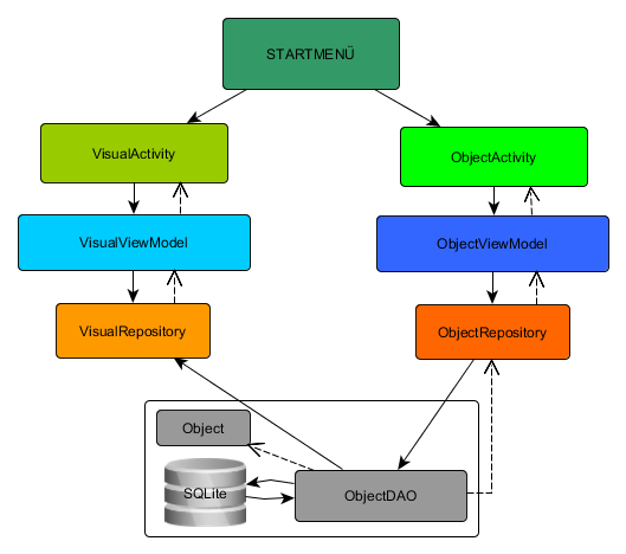
\includegraphics[width=13cm,height=13cm,keepaspectratio]{3Konzeption/Bilder/architektur_konzept.png}
    \caption{Konzeptionelle Software-Architektur}
    \label{pic:architectur}
\end{figure}
\pagebreak
\section{Softwarekonzept}
\label{chap:Softwarekonzept}
Nachdem die Architektur konzipiert und ein grobes Bild des entstehenden Systems geschaffen wurde, konnte die Konzeption des 
Softwaresystems beginnen. Hierbei werden die Kernfunktionen, sowie die Anforderungen und Ziele veranschaulicht.
\\ 
\linebreak 
Beim Starten der Applikation öffnet sich das Startmenü der Anwendung. Hier sind auf einen Blick zentral alle Funktionen, die das System 
unterstützt, übersichtlich geboten. Dort wird die Möglichkeit offeriert, die Scan-Phase (\ref{chap:Scan-Phase}) zu starten oder fortzuführen 
oder die Visualisierungs-Phase (\ref{chap:Visualisierungs-Phase}) nach erfolgtem Scannen zu starten. Dabei wird auch das Ziel verfolgt, den 
Nutzer nicht mit Informationen zu erschlagen, bzw. den Nutzer nicht unnötig zu verwirren und ohne große Probleme zu der eigentlichen Tätigkeit 
zu führen. Auch dient das Startmenü lediglich zur Navigation und leitet den Benutzer auf die von ihm gewählte Tätigkeit weiter.  
\subsection*{Scan-Phase}
Die oben genauesten beschriebene Scan-Phase (\ref{chap:Scan-Phase}) wird nochmals aufgegriffen. Mithilfe dessen wird die Konzeption dieser 
Kernfunktion auf Basis des Layouts und der darin geplanten Komponenten dargelegt.
\\ 
Grundsätzlich soll die Scan-Funktion eine Oberfläche enthalten, die die Wiedergabe des Kamerabildes gewährleistet. Dies soll mit einem 
speziellen \textit{ARCore-Fragment} umgesetzt werden, welches die Benutzeroberfläche überlagert und einen Großteil des Bildschirms einnimmt. 
Die Oberfläche soll zu folgenden Interaktionen zwischen Nutzer und Applikation, bzw. den darin enthaltenen dreidimensionalen Objekten 
dienen. Die vorgesehenen Interaktionen belaufen sich auf das Scannen der Umgebung durch die vom Smartphone gegebene Kamera, das Setzen von 
virtuellen Objekten auf die vom Nutzer vorgesehene Position und das hinzufügen von Informationen zu den jeweiligen Objekten. Unterhalb des 
\acs{AR}-Fragments soll eine \textit{Gallery} angezeigt werden, welche eine Auswahl der zu setzenden \acs{AR}-Objekte bietet und mit einem 
\textit{Button} pro Objekt versehen ist. So kann beim Klick auf ein Objekt-Button das dementsprechende \textit{3D asset} gerendert und auf 
dem \acs{AR}-Fragment angezeigt werden. Die Gallery kann im laufe der Entwicklung des Systems zu jeder Zeit um weitere \textit{3D assets} 
expandieren. Während des Renderings eines Objekts wird der Nutzer auf die Seite der Dateneingabe weitergeleitet, um speziell zu dem 
erzeugten Objekt Informationen eingeben zu können. Diese Informationen werden bei erneutem Wechsel zur 
Hauptseite samt der Daten der Position des Objekts in die SQLite Datenbank gespeichert, um den Voraussetzungen des Datenmodells 
(siehe Abschnitt \ref{chap:Datenmodell}) zu entsprechen.
\\
Ziel dieser Funktion ist, dem Nutzer eine simple Möglichkeit zu bieten das Umfeld zu scannen und Objekte an den vom Nutzer vorgesehenen 
Positionen zu platzieren. Dabei gilt es, die Anwendung so einfach wie möglich zu halten und das System auf die Kernaufgabe zu fokussieren.
\\ 
Abbildung (\ref{pic:anwendungsfall}) verdeutlich den konzipierten Inhalt der Scan-Phasen-Kernfunktion in einem Anwendungsfall-Diagramm, 
sodass oben aufgeführte Beschreibung zur optischen Darstellung mit den dahinterliegenden Klassen die Vorstellung und das Konzept präzisiert.
\\ 
\linebreak
Auf die zweite Kernfunktion wird in folgendem Abschnitt eingegangen, sowohl der Aufbau der Kernfunktion, als auch die damit einhergehenden 
Anforderungen und Zielsetzungen.
\subsection*{Visualisierungs-Phase}
Die zuvor erläuterte Visualisierungs-Phase wird in diesem Abschnitt seitens der Softwarekonzeption auf die Ziele, Anforderungen und 
Funktionen dargelegt.
\\ 
Ähnlich zur Scan-Phase gibt es bei dieser Funktion ein \acs{AR}-Fragment, welches das Kamerabild wiedergibt. Dieses Fragment soll sich 
über den gesamten Bildschirm erstrecken und sei zusätzlich mit zwei weiteren Buttons zu versehen. Diese werden in weiterem Verlauf 
präzisiert. Das Ziel dieser Kernfunktion ist die Darstellung aller vorhandenen, in der Datenbank gespeicherten, Gegenstände. Hierbei werden 
lediglich die Erzeugnisse, die in der Scan-Phase erstellt wurden, abgerufen und als neue Objekte gerendert. Dafür wird die Position in der 
SQLite Datenbank abgefragt und als Basis für das neue Objekt geladen. So können die vorhandenen Marker visuell dargestellt werden. Die 
Funktion an sich sieht keine Änderungen der bestehenden Objekte vor, dafür muss der Nutzer erneut in die Scan-Phase wechseln.
\\ 
Bevor der Benutzer von dem Startmenü zur Visualisierungs-Phase übergehen kann, soll ein Hinweis erscheinen, welcher sicherstellen soll das 
die Scan-Phase schon bereits mindestens einmal durchgeführt wurde. Damit wird sichergestellt, dass bereits Objekte existieren und angezeigt 
werden können. Denn ohne vorherigen Scan ist die Kernfunktion der Visualisierungs-Phase sinnlos.
\\
Neben dem \acs{AR}-Fragment gibt es zwei Button, den einen zum Navigieren auf die Scan-Methode, um bei Bedarf weitere Objekte 
hinzuzufügen und den zweiten zum Starten, bzw. erneuten Laden der Funktion. Damit wird die Abfrage der Daten, die in der Datenbank 
enthalten sind, gestartet und der Prozess des Objekterstellens, bzw. - renderns begonnen. Dadurch erscheinen alle bereits gespeicherten 
Objekte auf der Karte. Auf die Funktionen, Methoden und deren Umsetzung wird in Kapitel (\ref{chap:Umsetzung}) genauestens eingegangen.
\\ 
\linebreak
Dem Diagramm ist der zum jetzigen Zeitpunkt geplante Ablauf und Funktionsweisen des Unterstützungssystems zu entnehmen, dabei ist grob 
veranschaulicht, welche Möglichkeiten sich dem Nutzer bieten, um einen Überblick zu verschaffen anhand welcher Informationen die 
Applikation entwickelt wird. 
\begin{figure}[hbt!]
    \centering
    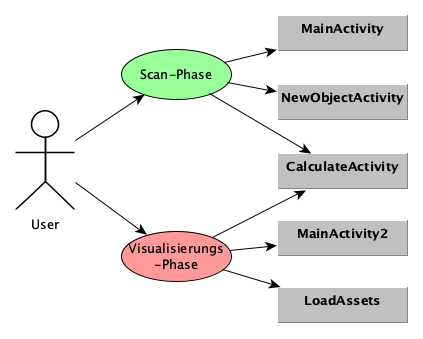
\includegraphics[width=13cm,height=13cm,keepaspectratio]{3Konzeption/Bilder/Anwendungsfalldiagramm.png}
    \caption{Anwendungsfall-Diagramm}
    \label{pic:anwendungsfall}
\end{figure}
\\ 
Nachdem auch das Softwarekonzept weitestgehend erarbeitet wurde, ging es um die Entscheidung, welches \acl{AR}-Framework für dieses Projekt 
ausgewählt wird. Nun wird die Evaluierung der Frameworks aufgegriffen, um einen Einblick in die Entscheidungsfindung zu gewähren.
\section{Auswahl des AR Frameworks}
\label{chap:Auswahl des AR Frameworks}
Mittlerweile gibt es eine enorme Auswahl an \acs{AR}-Frameworks, die alle unterschiedliche Präferenzen und 
Einsatzmöglichkeiten haben. Somit sind, auf den Bereich bezogen, Vor- und Nachteile im Vergleich von mehreren Frameworks nicht ausgeschlossen. 
Einige Alternativen wurden getestet und auf deren Brauchbarkeit evaluiert und analysiert. Dazu wurden Kriterien ausgearbeitet, die die 
Auswahl an Frameworks einschränken und nach Möglichkeit das passendste ergeben sollte: 
\pagebreak
\begin{enumerate}
    \item Eine performante Darstellung von Objekten.
    \item Möglichkeiten zur Positionsbestimmung.
    \item Eine aktive Community und stetige Weiterentwicklung des Systems.
    \item Möglichkeit zur Integration weiterer Technologien.
    \item Open Source-Projekt, um Flexibilität und weitestgehende Unabhängigkeit zu gewährleisten.
\end{enumerate}
Aufgrund der großen Anzahl an \acs{AR}-Frameworks war es nicht möglich alle in Betracht gezogenen Frameworks detailliert aufzuführen, 
lediglich die engere Auswahl der Tools wird aufgegriffen. 
\\ 
Nach ausführlicher Recherche wurden letzten Endes drei Frameworks in die nähere Auswahl aufgenommen, darunter \textit{vuforia}, 
\textit{ARToolKit} und \textit{Google ARCore}. Beweggründe zu dieser Entscheidung war die überwiegende 
Übereinstimmung zu zuvor aufgestellten Kriterien und Anforderungen. Alle Technologien konnten eine aktive und große Community, sowie eine 
aktive Entwicklung, bzw. Weiterentwicklung vorweisen. Zusätzlich bieten alle Frameworks viele Möglichkeiten zur Integration weiterer 
Technologien, um nach Belieben immer mehr Funktionen in das zu entwickelnde System übernehmen zu können. Die Performance der Technologien konnte 
in allen Aspekten überzeugen und ist unter einfachen Bedingungen mehr als ausreichend. Ein Kritikpunkt gegen die Verwendung von vuforia war 
die fehlende Verfügbarkeit des Quellcodes, da dieser unter kostenpflichtiger Lizenz steht und nicht als Open Source-Projekt gilt. Dadurch 
entfiel die Entscheidung für vuforia.
\subsection{ARToolKit}
ARToolKit ist ein \acs{SDK} zur plattformunabhängigen Entwicklung von \acl{AR} Anwendungen. Der Quellcode dieses Frameworks ist seit 2001 
frei verfügbar und ist vielseitig einsetzbar. Das Verfahren zur Positionsbestimmung durch Marker läuft schnell und robust. Marker wie in 
Abbildung \ref{pic:markerARpos} werden schnell und ohne Probleme erkannt. Jedoch gibt es diesbezüglich Einschränkungen die beachtet werden 
müssen, um eine zuverlässige und stabile Markererkennung zu gewährleisten, darunter Verdeckung des Markers, zu große Distanz von Kamera 
zu Marker, Blickwinkel auf den Marker und die Lichtverhältnisse des Umfelds. 
\\ 
Ein gravierender Nachteil des Frameworks für dieses Projekt ist die fehlende Unterstützung der Möglichkeit die 
Umgebung, bzw. das Umfeld zu erkennen und realisieren. So ist das Tracking nur über Marker, bzw. erweiterte 
markerbasierte Tracking-Methoden möglich. 
\\ 
Nach dieser Erkenntnis wurde auch dieses Framework als eher untauglich für die Verwendung in dem Projekt eingestuft. Möglicherweise 
gibt es einen Weg einen \acs{SLAM}-Algorithmus in Kombination mit ARToolKit zu verwenden, allerdings nicht ohne erweiterten Aufwand. 
Somit wurde dieser Weg eingestellt. 
\subsection{Google ARCore}
Google ARCore (siehe Abschnitt \ref{sec:arcore}) konnte bei der Analyse von sich überzeugen. Lediglich die Beschränkung der
Betriebssysteme auf \textit{Android} und \textit{iOS} war ein Nachteil, allerdings nicht von hoher Bedeutung. Der entscheidende Vorteil bei 
ARCore ist der unterstützende Algorithmus zur Umgebungserkennung. Des Weiteren ist Google ARCore ein Open-Source Projekt und befindet sich 
in kontinuierlicher Weiterentwicklung. Neben der stetigen Entwicklung hat sich eine große und aktive Community gebildet, die bei auftauchenden 
Problemen zur Stelle ist. Ein weiterer Vorteil sind die verschiedensten Möglichkeiten der Interaktion mit \acs{AR}-Objekten. Es gibt die 
klassische Markererkennung, die nicht nur mit Markern (siehe Abbildung \ref{pic:markerARpos}) sondern auch mit Bildern funktioniert, dem sogenannten
\textit{AugmentedImage}. Die Erkennung von Gesichtern, \textit{AugmentedFace} und die Erkennung von realen Punkten, Oberflächen und Gegenständen.
\\
\linebreak
Durch diese ganzen positiven Aspekte ist die Wahl des Frameworks auf das von Google entwickelte ARCore gefallen und wurde wegen den überzeugenden 
Grundlagen als Framework für dieses Projekt eingesetzt.

\section{Datenmodell}
\label{chap:Datenmodell}
Eine gute Basisstruktur der Datenspeicherung ist bei heutigem Datenverkehr ein wichtiger Bestandteil und genießt hohe Priorität. Deshalb ist 
es wichtig schon von Anfang an eine klare Richtlinie und Struktur zu erstellen, um bei nachträglichen Ergänzungen oder Änderungen zusätzlich so wenig 
Zeit wie möglich investieren zu müssen. Parallel zur Konzeption der Softwarearchitektur wurden Attribute zusammengetragen, die 
eine Basis der Informationen über verschiedenste Objekte aufgreifen soll. Mit den Objekten sind Gegenstände der realen Welt adressiert, die auch als 
virtuelle \acs{AR}-Objekte repräsentiert werden. Zu den Kernfunktionen, Scan- und Visualisierungs-Phase (\ref{chap:Scan-Phase} \& 
\ref{chap:Visualisierungs-Phase}) des Systems wurde entschieden, dass nur notwenige Daten, sogenannte Stammdaten, erhoben werden. Darunter 
der Name des Objekts, eine eindeutige ID, welche automatisch erzeugt wird, Größe, Alter, bzw. Baujahr des Gegenstands und virtuelle Position 
des \acs{AR}-Objekts. Die virtuelle Position ist durch die Scan-Phase gegeben und wird benötigt, um die Gegenstände in der 
Visualisierungs-Phase an der richtigen Stelle erneut einblenden zu können. 
\\ 
\linebreak 
Durch ein \acl{ERM} (\acs{ERM}), wurden die benötigten Daten zusammengetragen, aufgeführt und zu einem Modell konzipiert, um den Strukturen und 
Vorgaben der Datenmodellierung zu entsprechen und eine gute Basisstruktur zu erschaffen. Mit dieser Grundlage kann in Zukunft weitergearbeitet werden. 
Das Modell wurde mit der zuvor angesprochenen dritten Normalform umgesetzt, da diese die perfekte Balance in dem Datenmodell herstellt, um auftretende 
Probleme möglichst einfach zu lösen und diese nahe der Realität in das relationale Datenbankmodell einzupflegen. Dadurch kann eine Erweiterung des 
Datenmodells gewährleistet werden. Die Abbildung (\ref{pic:erm}) zeigt das erstellte ER-Modell auf und veranschaulicht die Modellierung. 
\\ 
\pagebreak
\begin{figure}[hbt!]
    \centering
    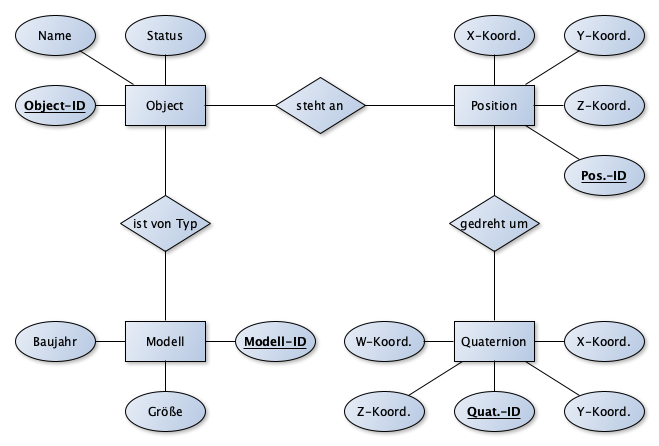
\includegraphics[width=15cm,height=15cm,keepaspectratio]{3Konzeption/Bilder/ERM_BA.png}
    \caption{Entity Relationship Datenmodell}
    \label{pic:erm}
\end{figure}
\\
Nach Beendigung des Datenkonzepts waren alle notwendigen Konzeptionen abgeschlossen. Diese wurden in Summe zusammengetragen und im Gesamten nochmals 
betrachtet und anhand neu gewonnener Kenntnisse überarbeitet und evaluiert. Da zu diesem Zeitpunkt alle Konzeptionen abgeschlossen 
waren, konnten diese zusammen analysiert und überdacht werden. 
\\ 
\linebreak
Nachdem diese Phase endgültig abgeschlossen war, konnte die Umsetzung des Konzepts und die 
Entwicklung des Systems starten. 